\section{Introduction to image processing}

\subsection*{Definition}
 Image processing is a structure determination technique that allows to get the 3D density map from a set of cryo-EM images of a particular macromolecule. Although different structural approaches can be followed to analyze the structures of macromolecules, this tutorial focuses on cryo-EM single particle analysis (SPA).  Fortunately, cryo-EM SPA is undergoing in this decade a resolution revolution that has allowed the structures of macromolecules to be solved at near-atomic resolution. 


 \subsection*{ Image processing workflow}
 
 The set of successive tasks aimed to get the 3D density map is known as image processing workflow. Main steps of the general workflow are detailed from top (movies) to bottom (refined volume) in the \ffigure{fig:image_processing_workflow}. Some of the tools required to perform the respective tasks are detailed in a non-exhaustive way on the right side of the Figure. All these methods have been integrated in \scipion to facilitate interoperability among different software packages, data tracking and reproducibility of results. 
 
 \begin{figure}[H]
 \centering
 \captionsetup{width=.8\linewidth}  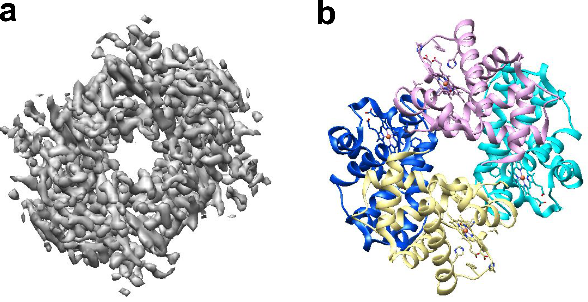
\includegraphics[width=0.55\textwidth]
  {{images/Fig1.pdf}}
  \caption{General image processing workflow for SPA \citep{scipion2016}. }
  \label{fig:image_processing_workflow}
  \end{figure} 
 
 The workflow considers as input the movie frames generated by the microscope. These movies should be global or locally aligned before computing the CTF of individual micrographs. \scipion allows to compare different CTF values obtained with distinct algorithms using the CTF consensus protocol. Once the CTF has been corrected, we are ready to extract individual particles of each micrograph by using different protocols of particle picking. As in the case of the CTF, we can retrieve the coordinates of each particle using different protocols of manual and automatic picking, and finally, estimate the agreement between all those methods through a consensus picking protocol. The screened particles are used for further processing. The next step involves the 2D classification of the individual selected particles. 2D classes derived from the last procedure contribute to generate the initial 3D map. The last part of the workflow includes 3D classification and 3D refinement tasks in order to iterative refine the initial 3D map.
 
 In this tutorial, we show all above mentioned processes of 3DEM processing, as well as the necessary tools to accomplish them, illustrating the combination of different EM software packages in \scipion.
 
% of model building every step of the general workflow will be considered, except the $de novo$ modeling step because the appropriate tools to accomplish this type of modeling are not still implemented in \scipion. 
 

  
